\chapter{Maintaining Room State \\
  \small{\textit{-- Evan Ciok, Sophia DiCuffa, Carson McManus}}
  \index{Chapter!room-state}
  \label{Chapter::RoomState}}

\section{Lost Balancer-Monolith Connections}

When a Balancer-Monolith connection is lost, clients connected to that monolith need to be handled appropriately. Otherwise, the accuracy of room state is compromised.
All client connections that are in rooms on the lost monolith are no longer valid, so they need to be disconnected and removed
from their rooms. From there, they can reconnect to a monolith with a new websocket connection to the balancer.

\section{Duplicate Rooms Across Monoliths\label{Section::duplicate-rooms-across-monoliths}}

Two monolith nodes should never have the same room loaded, as the load balancer should be directing all connections for a given room to the designated monolith using its preserved states.
In the case that this does happen, the system is then in a bad state and it must be resolved. The planned solution to this issue is to have the load balancer unload rooms that were not the
first instance of that particular room. This means that the duplicate instances would be unloaded and the clients could then rejoin the room in a healthy state. In order to accomplish this,
every room must have a timestamp associated with it, designating the time it was loaded. Then, in the case of duplication, the timestamps can be compared and the more recently loaded
instances can be handled appropriately. Following this, clients who were connected to a bad load of a room should be redirected to the home page where they can enter a new flow of room
creation or room joining.

\begin{figure}[!htb]
  \centering
  \scalebox{0.57}{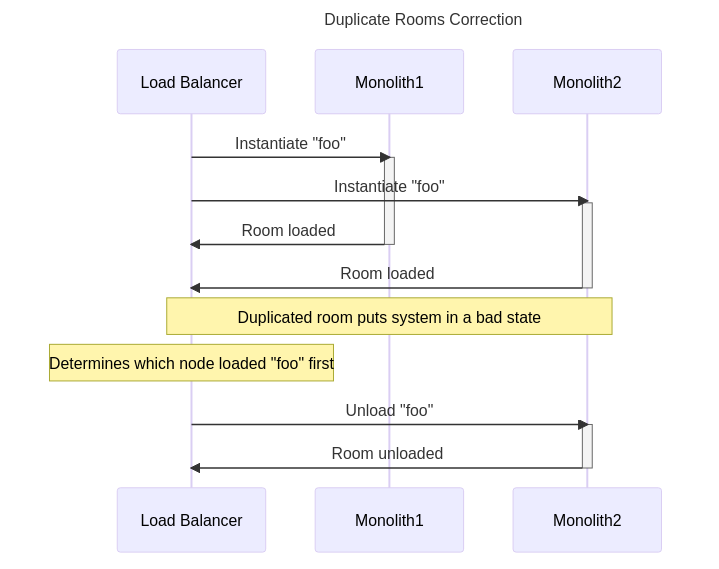
\includegraphics{Figures/duplicate-rooms.png}}
  \caption{\label{Figure::duplicate-rooms} Correcting system state following duplicate room instances.}
\end{figure}

\section{Maintaining Room State Across Service Restarts}

When OTT is deployed, the Monolith\index{monolith} is restarted. Also, heroku restarts OTT about every 24 hours. In order to make this not disruptive to end users, room state is constantly being flushed to redis. When OTT starts up, it gets a list of all the rooms that were loaded and tries to restore their state. The problem is that if a monolith restarts, then it will load all the rooms that are in redis. In a deployment with more than one monolith, this results in rooms existing on more than one monolith.

It's possible to simply allow the system to reach equilibrium using the mechanism described in Section \ref{Section::duplicate-rooms-across-monoliths}. However, this would result in a high memory usage on the Monolith\index{monolith} upon startup. It would also result in a lot of unnecessary network traffic and load on redis.

The solution is to use redis sets\cite{redis-sets} to manage the set of rooms currently loaded. This would guarentee that each room gets loaded only once, even if the resulting distribution of rooms is not optimal.

The system needs a mechanism to detect a cold start. This can be done by having all Monoliths touch a key in redis, \texttt{monoliths\_present}, every second, refreshing the expire time to 2 seconds in the future. If the key expires, then the system is in a cold start. If the system is in a cold start, monoliths that are starting up must start loading rooms from the \texttt{load\_queue}. Otherwise, they must not load any rooms.

However, this scheme implies that \texttt{load\_queue} needs to be maintained, and invalidated if a monolith crashes. Instead, each monolith should maintain it's own set of rooms that it has loaded, with the key in the format \texttt{rooms\_loaded:UUID}, with \texttt{UUID} replaced with a valid UUID. The UUID may be random, it does not need to be persistent across restarts. If the system is in a cold start, all monoliths that are starting up must merge all these sets into a new set called \texttt{load\_queue}, if it does not exist. The per-monolith room sets must expire at the same time room states expire.

\begin{figure}[!h]
  \centering
  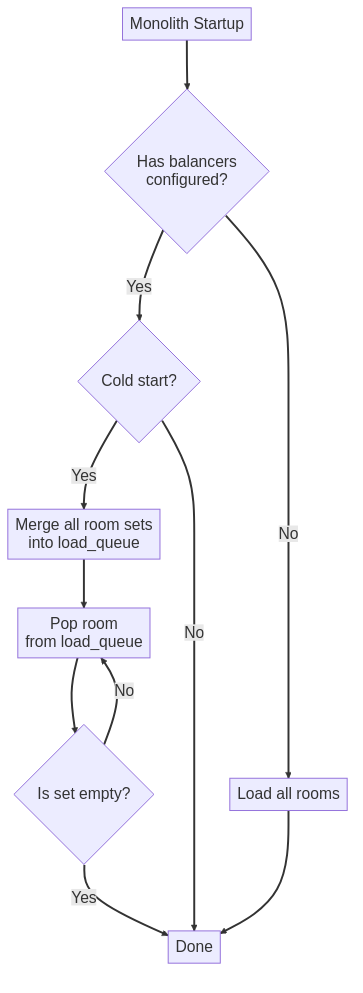
\includegraphics[width=0.35\textwidth]{Figures/monolith-startup.png}
  \caption{Flowchart for the Monolith's startup sequence}
  \label{Figure::monolith-startup}
\end{figure}

In order to avoid race conditions, the \texttt{WATCH} command inconjuction with redis transations via \texttt{MULTI} and \texttt{EXEC}\cite{redis-transactions} must be used. \texttt{WATCH} must come before \texttt{MULTI}, and it invalidates any commands that affects the watched keys when \texttt{EXEC} is called. The sequence of redis commands to perform this merge should be as follows:

\begin{verbatim}
	WATCH load_queue
	MULTI
	room_sets = KEYS rooms_loaded:*
	SUNIONSTORE load_queue $room_sets
	EXEC
\end{verbatim}